%%%%%%%%%%%%%%%%%%%%%%%%%%%%%%%%%%%%%%%%%%%%%%%%%%%%%%%%%%%
%
% RESULTS
%
%%%%%%%%%%%%%%%%%%%%%%%%%%%%%%%%%%%%%%%%%%%%%%%%%%%%%%%%%%%

%TODO: Explain results
%TODO: Explain the endogeneity DWH test used. Can't identify endogeneity?
%TODO: Elaborate on microsimulation 
%TODO: Reference graphs and tables in appendix. Conditional per type for instance.

%%%%%%%%%%%%%%%%%%%%%%%%%%%%%%%%%%%%%%%%%%%%%%%%%%%%%%%%%%%

\section{Results}
\subsection{Microsimulation Non-take-up}
Our microsimulation results indicate that the non-take-up-rate of BAföG, among theoretically eligible students ranged from approximately 50--70\% across the survey years 2007--2021, with an average of 60\%  (Table \ref{table:microsimulation-ntu}). 

These estimates are broadly in line with previous findings on non-take-up of social benefits in Germany, which generally falls between 40--67\%, depending on the program and time period (see Table \ref{table:NTU-studies}). 
While our estimates are broadly consistent with prior research, they are noticeably higher than the 36--40\% non-take-up rate for BAföG reported by \cite{herber_non-take-up_2019}, who also use SOEP survey data, but for the period 2002--2013.


\begin{table}[htbp]
\small
\centering
\begin{tabular}{l@{\hspace{2em}}r@{\hspace{2em}}r@{\hspace{2em}}r}
\toprule
\textbf{Year} & \textbf{Non-Take-Up} & \textbf{Take-Up Rate} & \textbf{Beta Error} \\
              & \(\Pr(\text{NTU} = 1 \mid \text{M} = 1)\) & \(\Pr(\text{TU} = 1 \mid \text{M} = 1)\) & \(\Pr(\text{TU} = 1 \mid \text{M} = 0)\) \\
\midrule
2007 & 60.6 & 39.4 & 13.6 \\
2008 & 63.5 & 36.5 & 17.1 \\
2009 & 61.0 & 39.0 & 18.6 \\
2010 & 60.9 & 39.1 & 17.7 \\
2011 & 53.8 & 46.2 & 16.1 \\
2012 & 51.5 & 48.5 & 18.9 \\
2013 & 50.0 & 50.0 & 15.9 \\
2014 & 55.1 & 44.9 & 16.1 \\
2015 & 64.0 & 36.0 & 12.6 \\
2016 & 56.5 & 43.5 & 12.4 \\
2017 & 62.6 & 37.4 & 10.1 \\
2018 & 63.9 & 36.1 & 15.3 \\
2019 & 67.5 & 32.5 & 11.7 \\
2020 & 63.7 & 36.3 & 13.6 \\
2021 & 66.7 & 33.3 & 12.3 \\
\midrule
\textbf{Average} & \textbf{59.7} & \textbf{40.3} & \textbf{15.0} \\
\bottomrule
\end{tabular}
\caption{\small{Non-Take-Up, Take-Up, and Beta Error Rates by Survey Year (\%). Non-take-up is the share of theoretically eligible students (\(M=1\)) who do not receive BAföG. The take-up rate is simply the complement, i.e., the share of eligible students who do receive BAföG \((1 - \Pr(\text{NTU} = 1 \mid M = 1))\). Beta error is the share of ineligible students (\(M=0\)) who nevertheless receive BAföG.}}
\label{table:microsimulation_ntu}
\end{table}


This discrepancy may be attributable to several factors, including differences in the estimation of theoretical eligibility. These factors include the specific SOEP variables used to capture income and reported BAföG receipt, the time periods under study (with our analysis covering 2007--2021, compared to \cite{herber_non-take-up_2019}, which covers 2002--2013), as well as other differences in the microsimulation design and modeling approach.

...

While there is some variation in non-take-up across years, NTU remains consistently quite high throughout the period. The rate fluctuates between a low of 50\% in 2013 and a high of around 68\% in 2019. Notably, the results show a decline from 2010 to 2013, which is then followed by a gradual upwards trend throughout the rest of the period. The increase in NTU in the years leading up to 2020 could potentially reflect behavioural or institutional factors such as changes in awareness, perceived complexity or attitudes toward debt, but it could also be partly driven by policy changes. Several BAföG reforms were introduced during this period, including increases in grant amounts and adjustments to income thresholds, which may have influenced both eligibility and perceived attractiveness of the program. Since the simulation accounts for these legal changes, the results capture not just behavioural responses but also how reforms may have affected take-up incentives over time.

\textcolor{red}{Maybe further elaborations belong in the discussion part?}

The second column in Table~\ref{table:microsimulation-ntu} shows the estimated beta error, which is the share of students who are classified as ineligible by the simulation but report receiving BAföG. On average, the beta error is about 15\% across the full period. This level of misclassification is in line with what other studies have found when working with survey data, where income reporting and timing mismatches are common issues \citep{frick_claim_2007}. While this level of beta error is not negligible, the simulation seems to capture eligibility status fairly well overall, even if some noise is unavoidable.

Taken together, the results suggest that a large share of eligible students do not take up BAföG, and that this has been the case fairly consistently over time. The high average non-take-up rate, around 60\%, points to persistent barriers such as lack of information or procedural hurdles. The financial attractiveness of BAföG may also be a factor. Although support amounts were increased at several points, the need-based allowances have consistently failed to keep pace with the actual cost of living for students \citep{staack_von_2017}. This could help explain why some students perceive the benefit as not worth the effort of applying. These findings underline the importance of outreach efforts and suggest that further reforms may be needed to make the program more accessible and appealing.

%TODO: Refer to the table of the distributions of reported bafög vs theoretical, see appendix for table.



\begin{figure}[htbp]
  \centering
  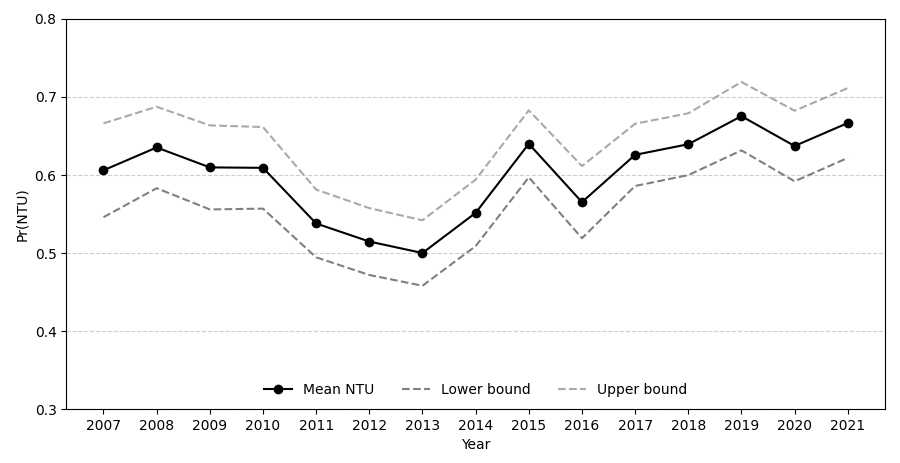
\includegraphics[width=0.75\linewidth]{ntu_bounds.png}
  \caption{Development of the probability of non-take-up from 2007--2021.}
  \label{fig:ntu_bounds_over_years}
\end{figure}


\subsection{Determinants of Non-take-up}

%TODO: Add some text here? 
% Could refer back to the method chapter where we go over the control variables

\subsubsection{Binary Choice Model}

To check the robustness of our findings, both logit and probit models are estimated and their average marginal effects (AMEs) are compared. 
As shown in Table~\ref{tab:logit_probit_lpm_results}, the results are very similar across the two models. 
The estimated effects have the same signs, similar magnitudes and are statistically significant in both cases. 
In particular, the simulated BAföG amount has a negative association with the probability of non-take-up. 
A 100~EUR increase in the simulated entitlement is linked to a decrease in the likelihood of non-take-up by about 2.9 to 3.0 percentage points. 
This supports the idea that students are more likely to apply when the potential benefit is higher.

To check the robustness of our findings, both logit and probit models are estimated and their average marginal effects (AMEs) are compared. As shown in Table~\ref{tab:logit_probit_lpm_results}, the results are very similar across the two models. The estimated effects have the same signs, similar magnitudes and are statistically significant in both cases. In particular, the simulated BAföG amount has a negative association with the probability of non-take-up. A 100~EUR increase in the simulated entitlement is linked to a decrease in the likelihood of non-take-up by about 2.9 to 3.0 percentage points. This supports the idea that students are more likely to apply when the potential benefit is higher.

As an additional check, we estimate a linear probability model (LPM), reported in Table~\ref{tab:logit_probit_lpm_results}. 
Although the LPM comes with known limitations, it allows for a straightforward interpretation of coefficients. 
The key results remain consistent. The marginal effect of the BAföG amount is estimated to be minus 2.1 percentage points per 100~EUR, and the direction and significance of the main explanatory variables remain stable.

All in all, the consistency of results across logit, probit, and LPM models suggests that the findings aren't sensitive to the choice of estimation method. This increases confidence in the reliability of the identified determinants of non-take-up.

...

\paragraph{Pseudo R-squared.} In models where the traditional R-squared is not defined, such as binary outcome models like logit and probit, researchers commonly use pseudo R-squared measures to get a sense of model fit. These statistics aim to provide an indication of how well the model explains the observed outcomes, though they are not directly comparable to the R-squared in linear regression. Pseudo R-squared values can help assess the explanatory power of a model, but they should be interpreted with care. Unlike the R-squared in OLS, pseudo R-squared values do not have a clear benchmark and are not directly comparable across different models or datasets. Because of this, they should be viewed more as descriptive tools rather than definitive measures of explanatory power. It is generally recommended to use them alongside other model diagnostics rather than relying on them alone \citep{ozili_acceptable_2023}.

%TODO: When we have made a decision on the exact details of the logit/probit and the measure of pseudo R squared then write more about that here (the value we get for pseudo R squared and how it should be interpreted in context of the model)


\begin{table}
\caption*{$\Pr(\mathrm{NTU} = 1 \mid \mathbf{X})$}
\renewcommand{\arraystretch}{1.25}
\centering
\begin{tabular}{lccccc}
\toprule
& \multicolumn{2}{c}{Logit} & \multicolumn{2}{c}{Probit} & LPM \\
& Coef. & AME & Coef. & AME & Coef. \\
\midrule
\multicolumn{6}{l}{\textbf{Main explanatory variables}} \\
Simulated BAföG amount$^{\circ}$ & -0.160*** & -0.029*** & -0.095*** & -0.030*** & -0.021** \\
 & (0.058) & (0.010) & (0.034) & (0.010) & (0.010) \\
\midrule
\multicolumn{6}{l}{\textbf{Controls: Demographics}} \\
Age & 0.099*** & 0.018*** & 0.058*** & 0.018*** & 0.037*** \\
 & (0.019) & (0.003) & (0.011) & (0.003) & (0.003) \\
Female & -0.059 & -0.011 & -0.020 & -0.006 & 0.004 \\
 & (0.256) & (0.047) & (0.149) & (0.046) & (0.046) \\
Has partner & 1.429* & 0.262* & 0.874** & 0.271** & 0.157* \\
 & (0.810) & (0.149) & (0.444) & (0.137) & (0.084) \\
Direct Migration background & -0.700* & -0.128* & -0.419* & -0.130* & -0.130* \\
 & (0.378) & (0.068) & (0.219) & (0.067) & (0.068) \\
Indirect Migration background & -0.689** & -0.127** & -0.407** & -0.126** & -0.121** \\
 & (0.299) & (0.053) & (0.179) & (0.054) & (0.058) \\
\midrule
\multicolumn{6}{l}{\textbf{Controls: Household and Socioeconomic Background}} \\
Living at parents’ home & -0.019 & -0.004 & -0.008 & -0.002 & 0.034 \\
 & (0.270) & (0.049) & (0.160) & (0.050) & (0.048) \\
Sibling claimed BAföG before & -0.554* & -0.102** & -0.321* & -0.100* & -0.107* \\
 & (0.285) & (0.051) & (0.171) & (0.052) & (0.056) \\
East background & -1.253*** & -0.230*** & -0.749*** & -0.232*** & -0.252*** \\
 & (0.313) & (0.052) & (0.186) & (0.054) & (0.061) \\
Parents are highly educated & -0.015 & -0.003 & 0.004 & 0.001 & 0.018 \\
 & (0.293) & (0.054) & (0.175) & (0.054) & (0.052) \\
\midrule
\multicolumn{6}{l}{\textbf{Controls: Behaviour}} \\
Patience & 0.030 & 0.006 & 0.015 & 0.005 & 0.005 \\
 & (0.065) & (0.012) & (0.040) & (0.012) & (0.012) \\
Impulsiveness & -0.039 & -0.007 & -0.021 & -0.006 & -0.009 \\
 & (0.068) & (0.012) & (0.042) & (0.013) & (0.012) \\
Risk Apetite & -0.022 & -0.004 & -0.014 & -0.004 & -0.002 \\
 & (0.037) & (0.007) & (0.021) & (0.007) & (0.006) \\
\midrule
McFadden Pseudo $R^2$ & \multicolumn{2}{l}{0.10} & \multicolumn{2}{l}{0.10} & \\
Likelihood Ratio Test & \multicolumn{2}{l}{53.33 (p = 0.00)} & \multicolumn{2}{l}{53.20 (p = 0.00)} & \\
Adjusted $R^2$ & & & & & 0.74 \\
F-statistic & & & & & 103.8 (p = 0.00) \\
Observations & \multicolumn{5}{l}{458} \\
\bottomrule
\end{tabular}
\caption{Logit, Probit, and LPM (Linear Probability Model) coefficients. Logit and Probit also report average marginal effects. Standard errors are in parentheses. The LPM is estimated via OLS with MacKinnon and White (1985) robust (HC3) standard errors.}
\label{tab:logit_probit_lpm_results}
\caption*{\small{Notes: Significance levels: $^{{*}} p < 0.1$, $^{{**}} p < 0.05$, $^{{***}} p < 0.01$. Robust standard errors clustered at the student level. $\circ$ Indicates per 100 EUR.}}
\end{table}



...

\paragraph{Interpretation of Average Marginal Effects from the Probit Model.} All interpretations below are based on the average marginal effects (AMEs) from the Probit model presented in Table 3.

Student age is found to be significantly associated with NTU of BAföG. 
On average, each additional year of age increases the probability of NTU by 2.8 percentage points, holding all other variables constant. 
Similarly, student income has a significant effect, as a 100 EUR increase in gross monthly income is associated with a 1.2 percentage point increase in the probability of NTU, suggesting that higher-earning students may be less inclined to rely on BAföG support. 
Parental income matters as well. A 100 EUR increase in parental gross monthly income is associated with a 0.6 percentage point increase in the probability of NTU. 

%TODO: Note: look better into why AME is positive for student income and negative parental income. It could be interpreted in the way that students that work are highly motivated individuals, "on average" more so than those who don't, which could make them more likely to make it through the rigorous application process. Herber et al. say something like that.

Other variables that have to do with family background were also found to have an effect. 
For example, having an older sibling who previously received BAföG reduces the probability of NTU by 9.6 percentage points on average, suggesting that familiarity with the system encourages take-up. 
Migration background is significant only for students with an indirect migration background (those born in Germany to foreign-born parents). 
For this group, the probability of NTU is 8 percentage points lower on average compared to those without a migration background.  
Gender, partnership status, and household size do not appear to significantly affect NTU.

Students from East Germany are much less likely to forgo BAföG than their West German counterparts. The results show that having an East German background decreases the probability of NTU by about 25.9 percentage points, on average. This substantial difference could reflect regional variation in attitudes towards public support or perceived entitlement.

Lastly, the estimated theoretical BAföG amount is negatively associated with non-take-up, suggesting that an expected higher amount makes you more likely to apply in the first place.


